% Chapter 4

\chapter{Experimental Results} % Main chapter title

\label{Chapter4} % For referencing the chapter elsewhere, use \ref{Chapter4} 
In this chapter we begin with a qualitative analysis of the posterior topic distributions generated by the DTM and inspect the historical significance and context of patents with particularly high inferred influence from the DTM. More quantitatively, we then present results from evaluating the coherence of each model's topics. Following the results of coherence testing we show the results of document classification via the document topic vectors produced by each of the three models. We conclude this chapter by presenting the performance of K-means clustering on each of the document vector spaces as measured by the metrics described in section \ref{DocumentClustering}.


%----------------------------------------------------------------------------------------
\section{Qualitative analysis of topics}
% Illustrate the progression of a topic through time
% Identify influential patents to a topic and assess their historical importance to the field.
%

%stream and damless patents, check out word progression
The experimental results show that both the DTM and DIM successfully identify latent topic structures consistent with known industry history. Take for instance a representative topic generated by the DTM. In particular, the topic most associated with the CPC subclass of patents pertaining to "Stream and Damless" hydro power (those with the label \keyword{YO2E 10$/$28}). Figure \ref{fig:areaplot} illustrates the mean topic vector for documents of this CPC subclass across epochs, primarily dominated by topic 4. If we inspect the top words from the inferred posterior distribution of this topic, shown in figure \ref{fig:wwttTopic4}, we see that while central words such as "water" and "power" maintain a high likelihood, words such as "float" experience an increase in likelihood as time progresses. 

% area chart of cumulative topic percentages in class over time. (i.e. add up all the vectors, normalize ot total amount, find percent, repeat for each epoch.)
\begin{figure}[!htb]
\centering
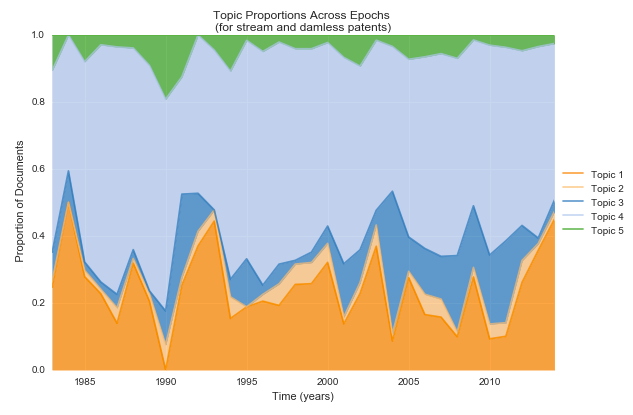
\includegraphics[width=130mm,scale=0.45]{Figures/areaplot2}
\decoRule
\caption[areaplot]{Proportion of topics at each epoch for patents relating to stream and damless hydro electric technology}
\label{fig:areaplot}
\end{figure}

% This parallels an increase in offshore floating barge popularity 
To understand why this might be the case we reviewed the known history of stream and damless hydro technology, and found that increase in the word "float" is of particular interest as it parallels closely the development of the wave and tidal energy industry both in the UK and globally. Vertical cross flow turbines such as the Gorlov turbine, patented in 2001, contributed to a rise in the popularity of floating barges for tidal power, a technology that represents the current norm of tidal current development \parencite{KhanOES}. Closely following this the European Marine Energy Centre (\keyword{EMEC}) was founded in 2003 and since then has supported the deployment of more wave and tidal energy devices than at any other single site in the world. This substantiates the linguistic trends we observe in Topic 4 and offers an explanation as to the rise in the estimated posterior mean number of occurrences of words such as "power" and "float" after 2003.

% also reflected in the importances of certain patents
Additionally, inspecting the patents in the "Stream and Damless" subclass that were estimated by the DIM as having a particularly high influence to Topic 4 reveals a similar narrative. During the same period of growth for barge based systems as discussed above, beginning around the year 2000, we see the DIM infer linguistic importance to related patents. For instance, a buoyancy pump in 2000, an energy generating method and device for utilizing buoyancy in 2006 and a cross flow hydraulic turbine in 2007 all received the largest influence scores of their epoch, a metric shown to correlate with forward citation rates \parencite{icml2010_GerrishB10}. In this way we are able to identify individual patents likely to have had an influence on the terminology of the field in which they were published \emph{without} knowledge of citation rates, that is, solely through analyzing language use. 

%posterior distribution of the corpus' patent influences


% word distributions of topic 4 over time plot (the topic most closely associated with the cpc label 28)
\begin{figure}[!htb]
\centering
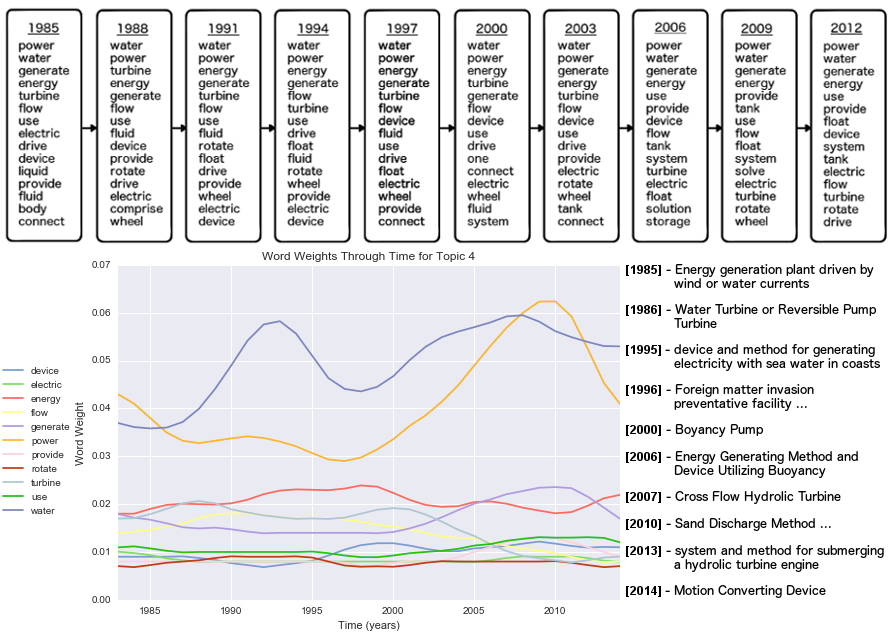
\includegraphics[width=130mm,scale=0.45]{Figures/Topic4}
\decoRule
\caption[wwttTopic4]{(top) The top fifteen words from the inferred posterior distribution of Topic 4 at three year lags. (bottom) The posterior estimate of the frequency as a function of year of words from Topic 4. (right) Patents of linguistic influence to topic across epochs as estimated by the DIM.}
\label{fig:wwttTopic4}
\end{figure}

%----------------------------------------------------------------------------------------
%\section{DIM Results and Insights}
%\subsection{Influence Metric}
%\subsubsection{validating influential patents}
%\subsubsection{correlation with forward citations}
%\subsubsection{correlation with page-rank}

%----------------------------------------------------------------------------------------
\section{Coherence Testing}


The aggregated topic coherence results of the tuned models are shown in Table \ref{tab:coherences} for the DTM, DIM and LDA models respectively.

The DTM proved superior in all coherence measures except Umass, the measure that correlates the least with human judgement by a considerable amount. Not only did the DTM regularly obtain the highest coherence scores, it did so by a large margin obtaining nearly double the c$\_$uci score obtained by static LDA. We attribute this performance to the unique structure of the DTM. Rather than enforcing "one size fits all", broad sweeping topics across the whole corpus, each epoch receives in effect its own LDA model. Each of these individual LDA models inherits a set of variational parameters $\alpha$ and $\beta$, controlling its document topic proportions and topic word distributions respectively, from the previous time step perturbed by Gaussian noise. The result is a richer posterior compared to static LDA that allows for a 'tighter fit' to the true posterior. This of course takes longer to train but is demonstrably worth the performance increase.


The DIM also tended to outperform static LDA, though to a slightly lower degree than DTM, even yielding the highest U$\_$mass score. It is interesting to observe that the DIM obtained coherence scores similar to, but consistently smaller than, that of its counterpart the DTM. This is again due to the structure of the model. The DIM borrows a similar Markov chain structure of term distributions in order to capture drifts in probabilities over the course of the collection but with a critical difference. While the topic word distribution natural parameters $\beta$ are passed along at each time step the DIM does not chain its document topic proportion natural parameters $\alpha$. Each time step's LDA operates under the same $\alpha$ parameters which weakens its ability to superresolve temporal topic trends. This explains the increased performance of the DIM over traditional LDA, and reduced performance compared to the DTM. 

\begin{table}[!htb]
\caption[Coherences]{The coherence values attained by each model}
\label{tab:coherences}
\centering
\begin{tabular}{l l l l l}
\toprule
\tabhead{Model} & \tabhead{c$\_$v} & \tabhead{c$\_$uci} & \tabhead{c$\_$npmi} & \tabhead{u$\_$mass} \\
\midrule
LDA & .5021 & .1904 & .0750 & -1.6283 \\
DIM & .5581 & .2865 & .1011 & \keyword{-1.3478} \\
DTM & \keyword{.5980} & \keyword{.4373} & \keyword{.1213} & -1.6688 \\
\bottomrule\\
\end{tabular}
\end{table}

Results are similar when looking at coherence across epochs rather than aggregated coherence scores contained in figure \ref{fig:EpochCoherences}. As the static LDA produced only a single set of topics for the entire corpus its coherence scores remain constant. The DTM however provided unique topics across epochs and thus obtained a sequence of coherence scores. This sequence of scores proved relatively constant and again remained above those of the static LDA model for all measures except Umass.
 
 %Again, Umass gives less conclusive results than the other metrics. 

\begin{figure}[!htb]
\centering
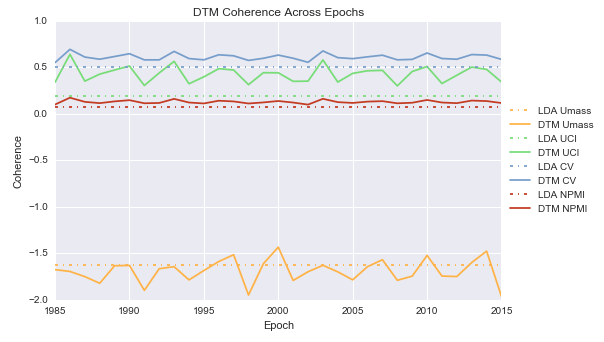
\includegraphics[width=130mm,scale=0.45]{Figures/DTMCoherences}
\decoRule
\caption[EpochCoherences]{Coherence scores for the DTM and LDA across epochs}
\label{fig:EpochCoherences}
\end{figure}


%----------------------------------------------------------------------------------------
\section{Classification Results}

% they cite the normalized mutual information equation! use those!
The clustering result is evaluated by comparing the Normalized mutual information (Xu et al. 2003; Cai et al. 2008) [NEED TO ACTUALLY CITE]
%Xu, W., Liu, X., & Gong, Y. (2003). Document clustering based on non-negative matrix factorization. In
%SIGIR ’03: Proceedings of the 26th annual international ACM SIGIR conference on research and
%development in informaion retrieval (pp. 267–273). New York, NY, USA: ACM.
%Cai, D., Mei, Q., Han, J., & Zhai, C. (2008). Modeling hidden topics on document manifold. In
%J. G. Shanahan, S. Amer-Yahia, I. Manolescu, Y. Zhang, D. A. Evans, A. Kolcz, K.-S. Choi, &
%A. Chowdhury (Eds.), CIKM (pp. 911–920). ACM.

\section{Clustering Results}

